\documentclass[11pt]{article}
\usepackage[utf8]{inputenc}
\usepackage{lingmacros}
\usepackage{tree-dvips}
\usepackage{enumitem}
\usepackage{graphicx}
\usepackage{lmodern}
\usepackage[T1]{fontenc}
\usepackage[bottom]{footmisc}
\graphicspath{ {./images/} }

\newenvironment{remerciements}
  {
   \thispagestyle{empty}% no header and footer
   \vspace*{\stretch{1}}% some space at the top
   \itshape             % the text is in italics
  }
  {\par % end the paragraph
   \vspace{\stretch{3}} % space at bottom is three times that at the top
   \clearpage           % finish off the page
  }

\title{Monitoring des données BRAMS et détection automatique des échos de météore}
\author{Miguel Antoons}

\begin{document}

\begin{titlepage}
    \begin{center}
        
\includegraphics[]{logo_ephec.png}\\
        \Large
        \textbf{Technologie de l'Informatique}\\
        \large
        Avenue du Ciseau 15\\
        1348 Ottignies
    \end{center}

    \vspace*{\stretch{1.0}}

    \begin{center}
        \line(1,0){350}\\
        \LARGE\textbf{Monitoring des données BRAMS et détection automatique des échos de météore}\\
        \line(1,0){350}\\
        \vspace{0.5cm}
        \LARGE\textit{Miguel Antoons}\\
        \vspace{0.5cm}
        \Large\textbf{Rapporteur}\\
        \Large\textit{Monsieur Arnaud Dewulf}
    \end{center}

    \vspace{0.14cm}

    \begin{center}
        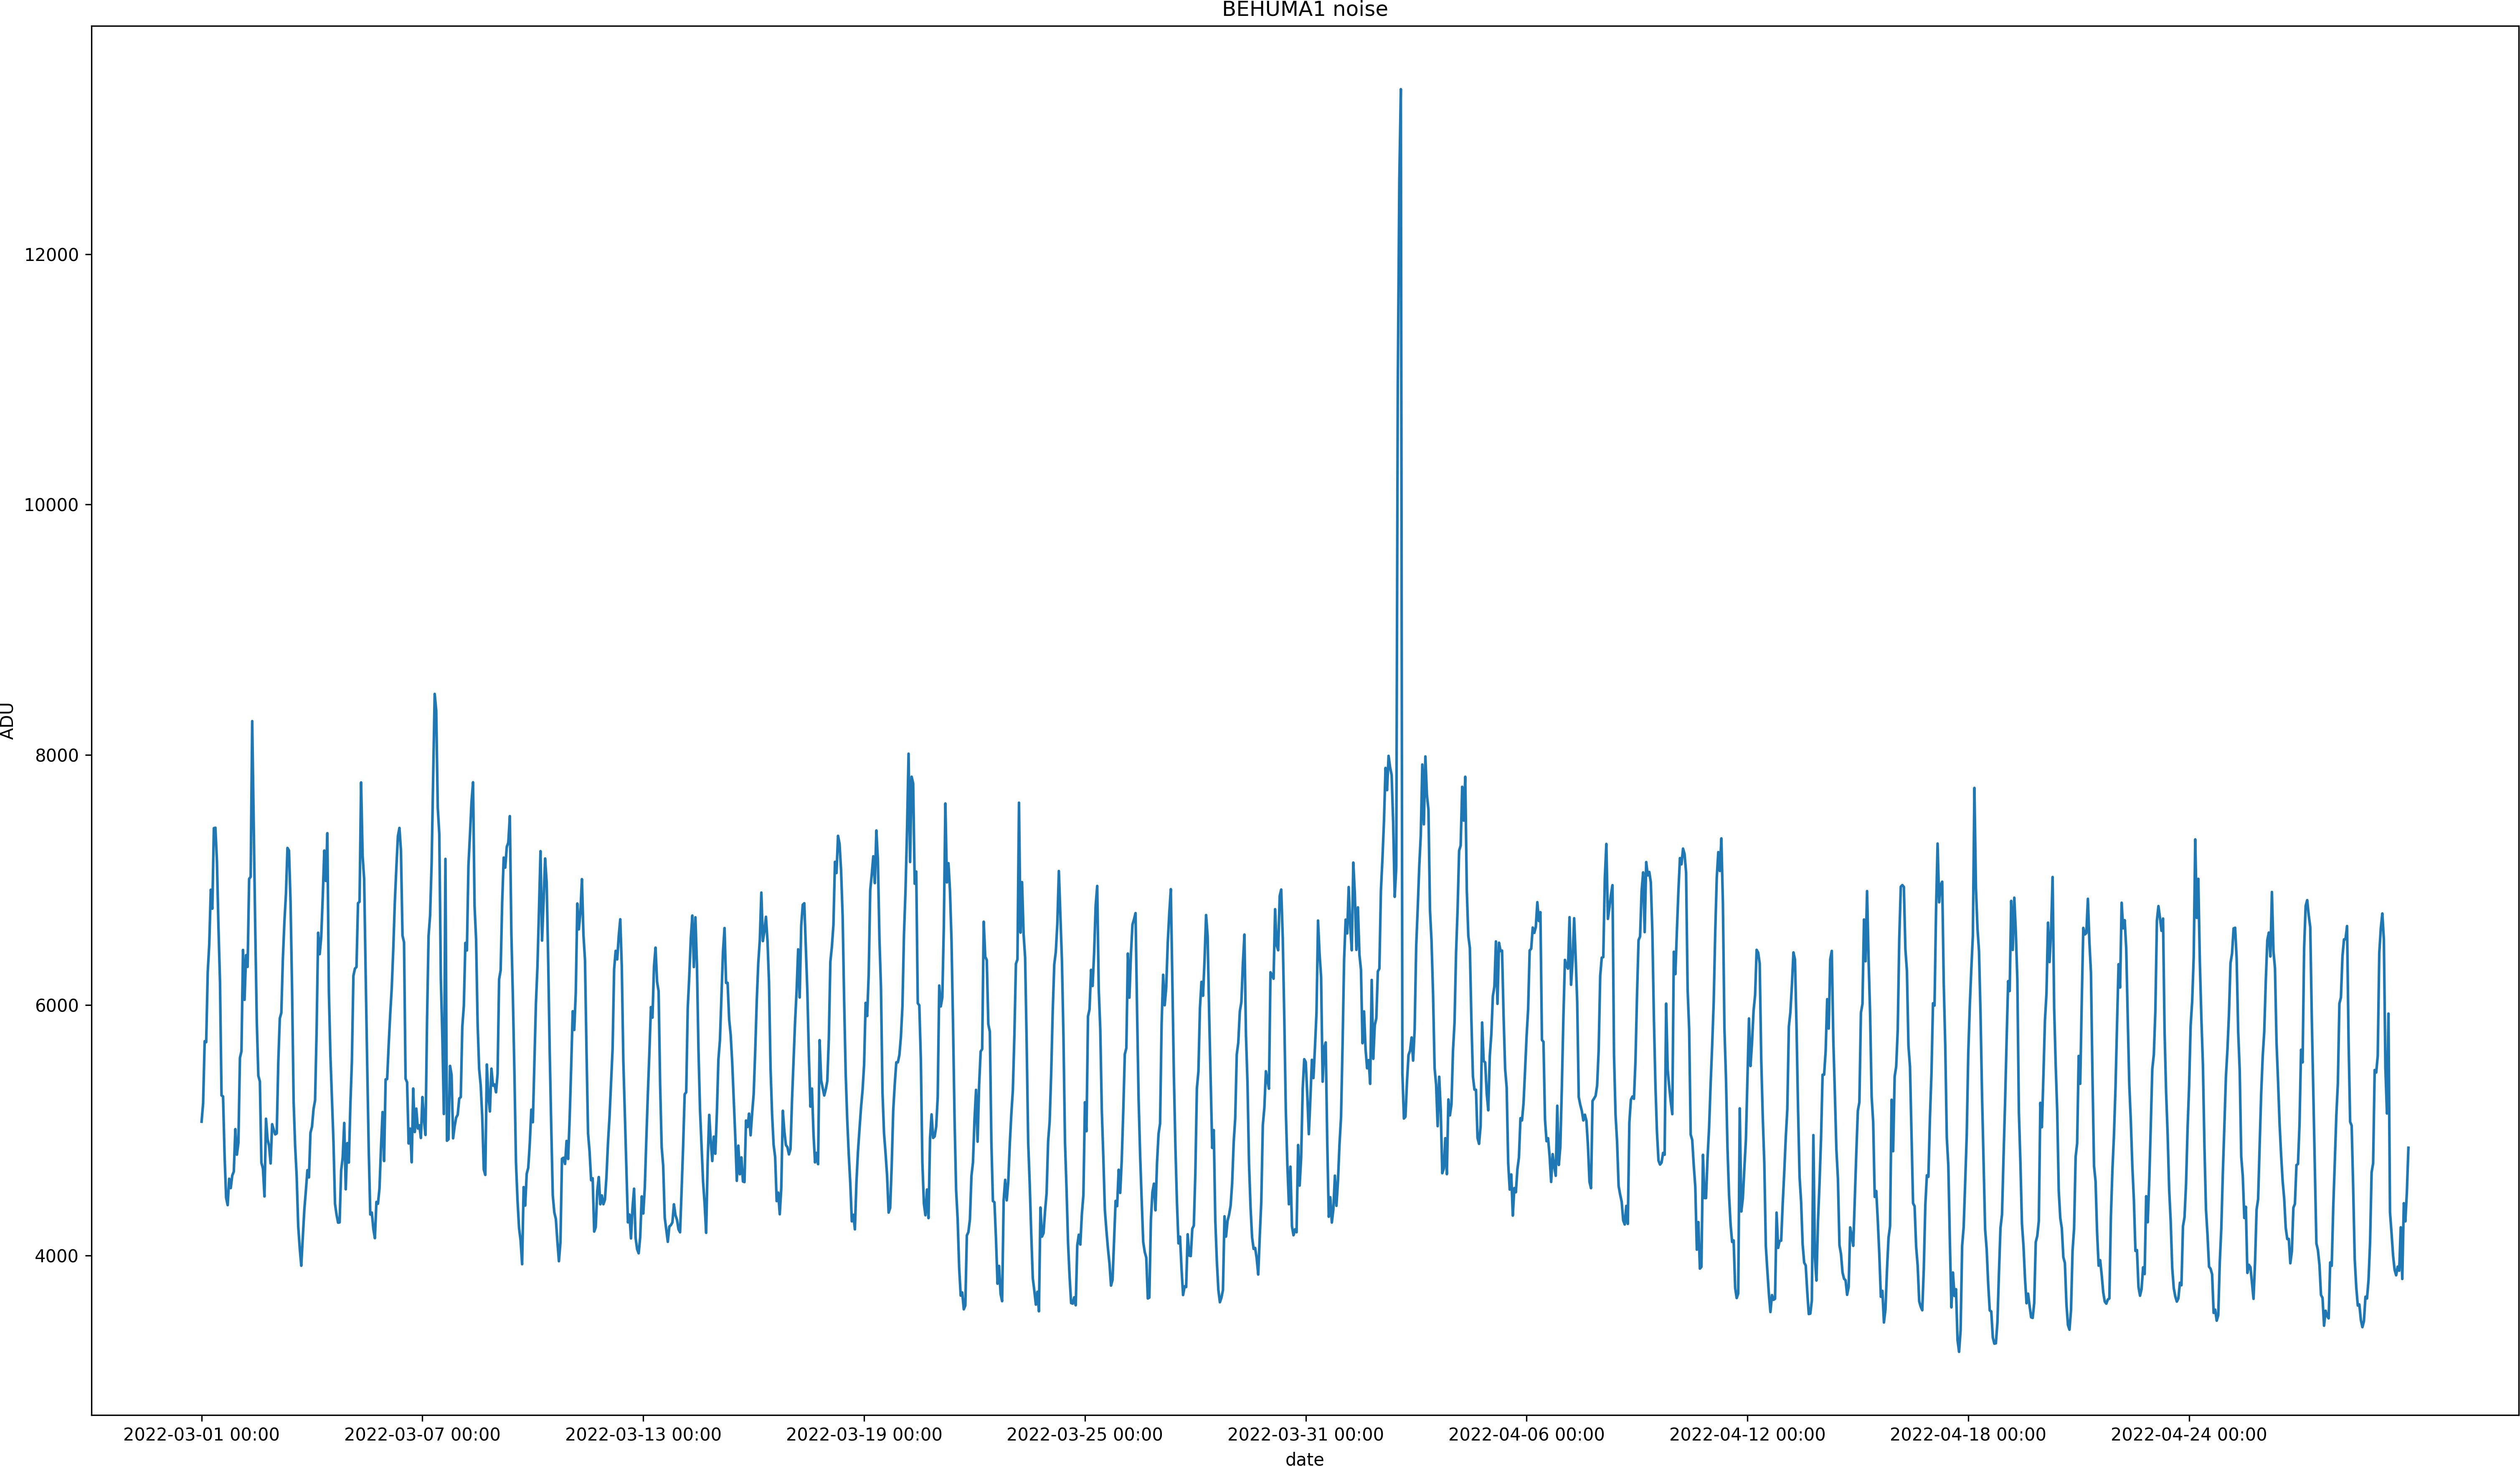
\includegraphics[scale=0.225]{page_garde.png}\\
        \vspace{0.14cm}
        \textit{2021-2022}
    \end{center}



    \vspace*{\stretch{2.0}}
\end{titlepage}

\section*{Remerciements}
\begin{remerciements}

    Je tiens tout d'abord à remercier toutes les personnes qui m'ont aidé à réaliser ce projet de fin d'études.\\
    \par
    En commençant par mon professeur rapporteur, à qui j'ai pu poser mes questions en cas de besoin et qui s'est assuré que tout se passe bien tout au long du projet.\\
    \par
    Ensuite, je voudrai remercier Mr Hervé Lamy pour avoir proposé ce sujet de fin d'études, mais également pour m'avoir expliqué, de façon claire et précise, toutes les notions qui nécessitaient des explications.\\
    \par
    Je tiens également à remercier Mrs Antoine Calegaro et Michel Anciaux, qui m'ont guidé quand c'était nécessaire et qui m'ont conseillé durant le projet de fin d'études.\\
    \par
    Enfin, je voudrais exprimer ma reconnaissance envers toutes les personnes qui m'ont conseillé sur, et ont relu ce rapport de projet de fin d'études.
\end{remerciements}

\newpage

\tableofcontents

\newpage

\section{Introduction}

\subsection{Le projet BRAMS}

Lancé en 2010 par Monsieur Hervé Lamy à l'Institut Royal d'Aéronomie Spatiale de Belgique, le projet BRAMS (Belgian RAdio Meteor Stations) à pour but de collecter et stocker des données relatives à des objets rentrant dans l'atmosphère belge et, plus précisément, des météores.
Ces données pourront ensuite être analysés afin de retrouver la trajectoire, la vitesse ou encore la masse d'un ou de plusieurs météores.\\
\\
Afin d'accomplir ce but, le projet BRAMS dispose d'un réseau de stations nommé le réseau BRAMS.
Pour comprendre le fonctionnement du réseau BRAMS, la première chose à savoir est : lorsqu'un météore passe dans l'atmosphère, il laisse derrière lui une trainée ionisée.
Cette trainée à la propriété de réfléchir les ondes radio.
Dans la plus grande partie des cas cette réflexion se fait en un seul point le long de la trajectoire, phénomène qui s'appelle la réflexion spéculaire (illustré à la figure 1).
La position point, nommé le point de réflexion spéculaire, dépend notamment du positionnement de l'émetteur, du positionnement du récepteur et de la trajectoire du météore.\\
\\
% ! explain station types
Pour exploiter le phénomène de la réflexion spéculaire et réussir à détecter les météores à l'aide d'ondes radios, le réseau BRAMS fonctionne de la façon suivante :
\begin{enumerate}
    \item Un émetteur, situé à Dourbes, transmet de façon continue un signal à une fréquence de 49.97 MHz.
          Ce signal est émis en direction du ciel et peut être réfléchi sur des trainées ionisées dans le sillage des météores.
    \item Lorsque le signal est réfléchi, il peut être détecté par une ou plusieurs stations réceptrices faisant partie du réseau BRAMS.
          Un signal calibreur est alors additionné au signal venant du ciel.
          Ce signal est injecté à 49.9705 MHz, c'est-à-dire 500 Hz plus haut que le signal direct.
          Il dispose d'une amplitude fixe et sert de référence d'amplitude pour le reste du signal.
          La station réceptrice décale ensuite le signal direct de 49.97 MHz vers une fréquence de 1 kHz.
    \item Ensuite, la station réceptrice enregistre l'ensemble du signal dans un fichier son de type WAV\footnote{Waveform Audio File}.
          Le signal est échantillonné à une fréquence de 5512 ou 6048 Hz dépendant du type de station.
\end{enumerate}


\end{document}